\chapter{Appendices}

This Chapter provides all the appendixes we mentioned during our thesis. Their original files can be accessed on the thesis repository~\cite{mt-forge} as well.

% -----------------------------------------------------------------------------
\newappendix{Specifications Document}
\label{appendix:specifications}

The next twenty-nine pages present the specifications document that has been defined for this thesis.


\includepdf[pages=-]{03-tail/appendices/specifications.pdf}

% -----------------------------------------------------------------------------
\newappendix{Guide Content}
\label{appendix:guide}

%TODO
The next fifty pages present the spreadsheet file acting as the dataset that has been defined during this thesis.

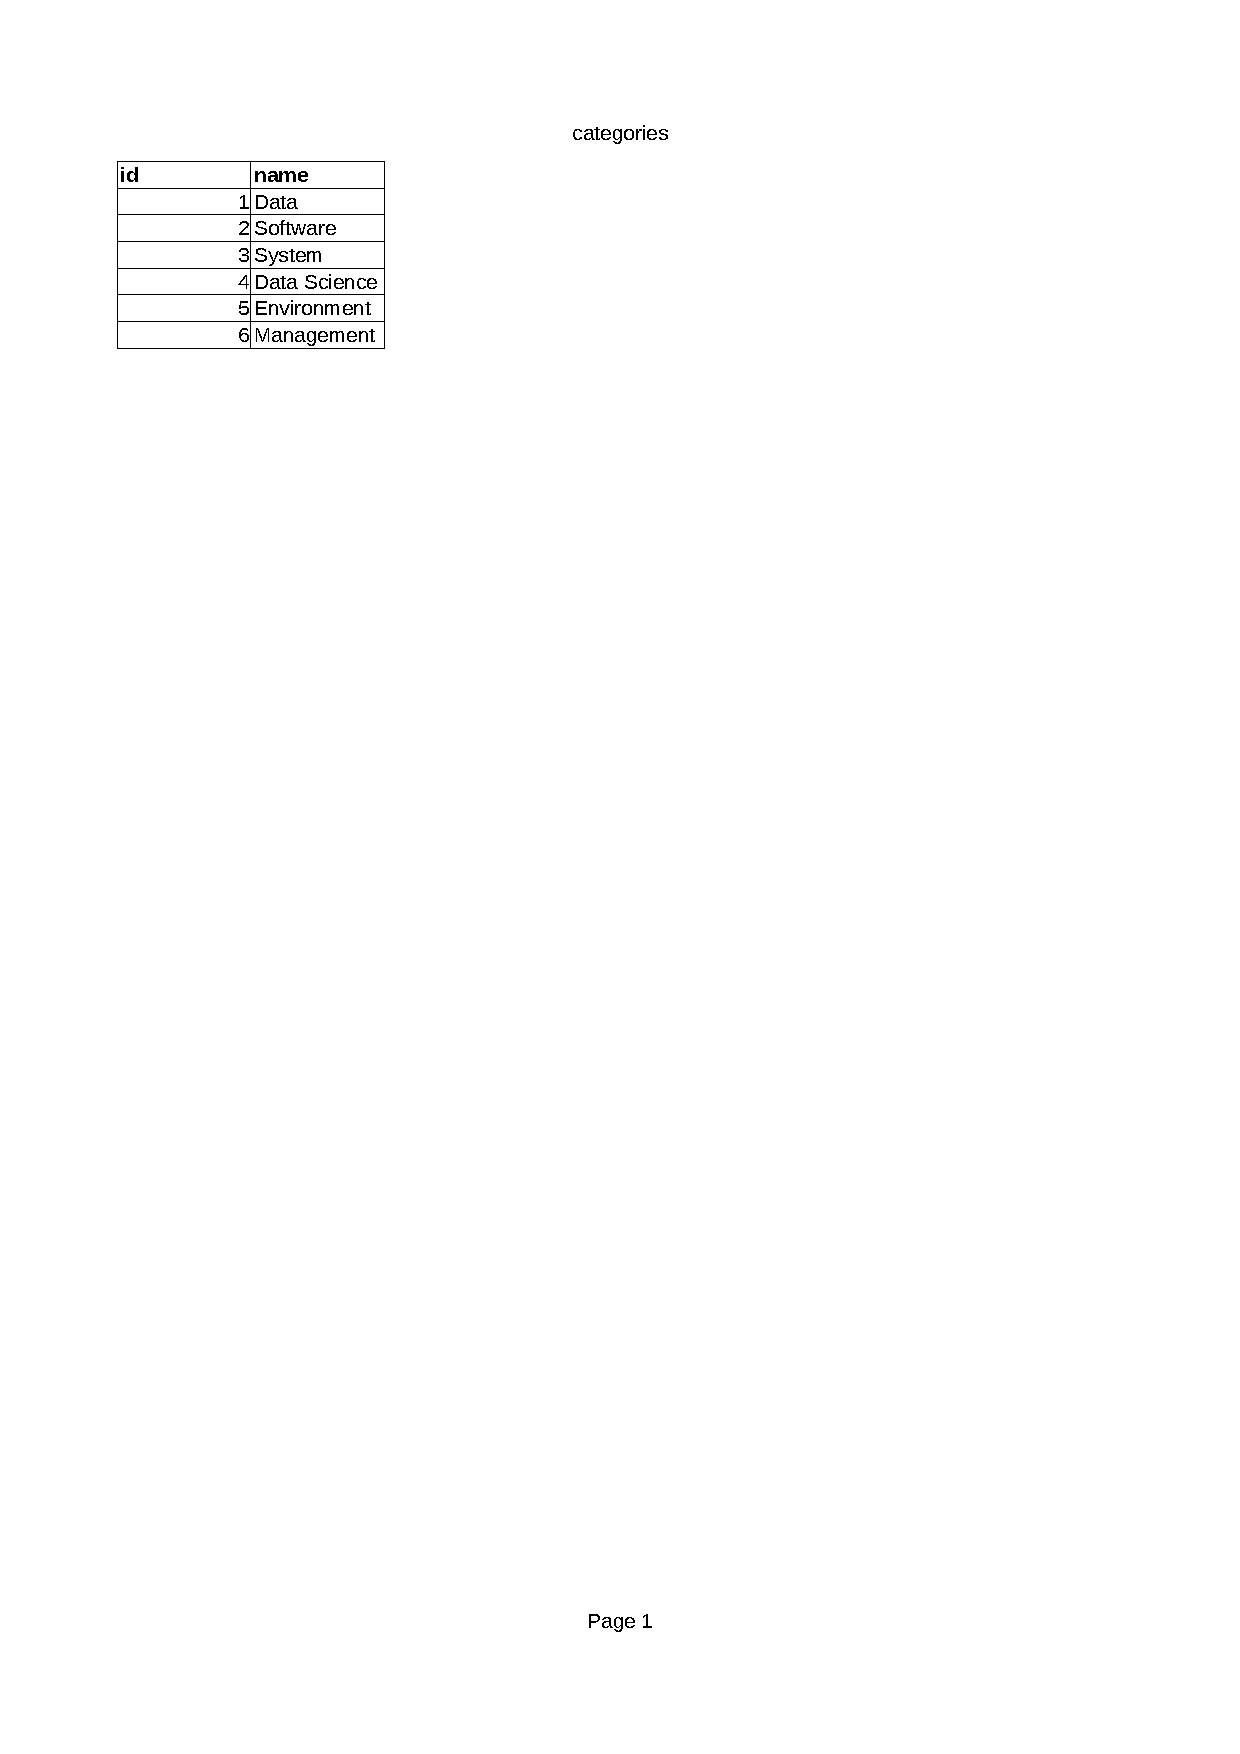
\includepdf[pages={-},fitpaper,rotateoversize]{03-tail/appendices/dataset.pdf}

% -----------------------------------------------------------------------------
\newappendix{Software Tests}
\label{appendix:tests}

\captionsetup[table]{list=no}

% Counters 
\newcounter{testsdatacounter}
\newcounter{testsappcounter}

The results of the conducted software tests are summarized in this appendix.

\begin{hyphenrules}{nohyphenation}
	\begin{table}[ht]
		\begin{center}
			\begin{tabularx}{\textwidth}{l|p{4cm}Xc}
				\toprule[0.8mm]
				\textbf{ID} & \textbf{Action} & \textbf{Expected result} & \textbf{Result} \\
				\midrule[0.8mm] 
				\stepcounter{testsdatacounter}
				1.\thetestsdatacounter & Run script with valid arguments & The arguments are passed to the script and used by it & \cellcolor{green!25}OK \\
				\midrule 
				\stepcounter{testsdatacounter}
				1.\thetestsdatacounter & Run script with invalid arguments & The script exits after showing the arguments & \cellcolor{green!25}OK \\
				\midrule 
				\stepcounter{testsdatacounter}
				1.\thetestsdatacounter & Run script without arguments & The script exits after showing the arguments & \cellcolor{green!25}OK \\
				\midrule 
				\stepcounter{testsdatacounter}
				1.\thetestsdatacounter & Run script with the \texttt{help} argument & The script exits after showing the arguments & \cellcolor{green!25}OK \\
				\midrule 
				\stepcounter{testsdatacounter}
				1.\thetestsdatacounter & Run script with as invalid \citeproper{ODS} file & The script exits after showing the reason & \cellcolor{green!25}OK \\
				\midrule 
				\stepcounter{testsdatacounter}
				1.\thetestsdatacounter & The \citeproper{ODS} file has an invalid attribute & The attribute is not processed & \cellcolor{green!25}OK \\
				\midrule 
				\stepcounter{testsdatacounter}
				1.\thetestsdatacounter & The \citeproper{ODS} file has an invalid value & The script shows the error & \cellcolor{green!25}OK \\
				\midrule 
				\stepcounter{testsdatacounter}
				1.\thetestsdatacounter & The hash is calculated based on the guide content & The hash is valid & \cellcolor{green!25}OK \\
				\bottomrule[0.8mm]
			\end{tabularx}
		\end{center}
		\caption*{Data conversion tests}
	\end{table}
\end{hyphenrules}

\begin{table}[ht]
    \begin{center}
        \begin{tabularx}{\textwidth}{l|XXc}
            \toprule[0.8mm]
            \textbf{ID} & \textbf{Action} & \textbf{Expected result} & \textbf{Result} \\
            \midrule[0.8mm] 
			\stepcounter{testsappcounter}
            2.\thetestsappcounter & Click on the evaluation button. & The \texttt{ExplanationView} page opens. & \cellcolor{green!25}OK \\
            \midrule 
			\stepcounter{testsappcounter}
            2.\thetestsappcounter & Click on the restoration button. & The \texttt{ResorationView} page opens. & \cellcolor{green!25}OK \\
            \midrule 
			\stepcounter{testsappcounter}
            2.\thetestsappcounter & Click on the report button. & The report \gls{pdf} file opens in another tab. & \cellcolor{green!25}OK \\
            \midrule 
			\stepcounter{testsappcounter}
            2.\thetestsappcounter & Click on the \gls{pwa} browser titles. & Additional installation information is shown. & \cellcolor{green!25}OK \\
            \midrule 
			\stepcounter{testsappcounter}
            2.\thetestsappcounter & Click on the \gls{pwa} links. & Links are opened in another browser tab. & \cellcolor{green!25}OK \\
            \bottomrule[0.8mm]
        \end{tabularx}
    \end{center}
    \caption*{Application tests on the \texttt{HomeView} user interface}
    \label{table:app_tests_ui_homeview}
\end{table}

\begin{hyphenrules}{nohyphenation}
\begin{table}[ht]
    \begin{center}
        \begin{tabularx}{\textwidth}{l|p{3.2cm}Xc}
            \toprule[0.8mm]
				\textbf{ID} & \textbf{Action} & \textbf{Expected result} & \textbf{Result} \\
				\midrule[0.8mm] 
				\stepcounter{testsappcounter}
				2.\thetestsappcounter & Click on the upload form. & A system modal window opens to select a \gls{json} file. & \cellcolor{green!25}OK \\
				\midrule 
				\stepcounter{testsappcounter}
				2.\thetestsappcounter & Click on the upload submit button. & The integrity of the \gls{json} file is verified, the progress or results are saved into the store and the assessor is redirected to either the \texttt{EvaluationView} page or the \texttt{ResultsView} page. & \cellcolor{green!25}OK \\
				\bottomrule[0.8mm]
        \end{tabularx}
    \end{center}
    \caption*{Application tests on the \texttt{RestoreView} user interface}
    \label{table:app_tests_ui_restoreview}
\end{table}
\end{hyphenrules}

\begin{hyphenrules}{nohyphenation}
	\begin{table}[ht]
		\begin{center}
			\begin{tabularx}{\textwidth}{l|p{4cm}Xc}
				\toprule[0.8mm]
				\textbf{ID} & \textbf{Action} & \textbf{Expected result} & \textbf{Result} \\
				\midrule[0.8mm] 
				\stepcounter{testsappcounter}
				2.\thetestsappcounter & Click on the text to change guide content. & Additional information and an upload form are shown. & \cellcolor{green!25}OK \\
				\midrule 
				\stepcounter{testsappcounter}
				2.\thetestsappcounter & Click on the upload form. & A system modal window opens to select a \gls{json} file. & \cellcolor{green!25}OK \\
				\midrule 
				\stepcounter{testsappcounter}
				2.\thetestsappcounter & Click on the upload submit button. & The integrity of the \gls{json} file is verified, the guide content is saved into the store, and the assessor is redirected to the \texttt{EvaluationView} page. & \cellcolor{green!25}OK \\
				\midrule 
				\stepcounter{testsappcounter}
				2.\thetestsappcounter & Click on an item of the guide example. & If at least one description exists for the item, the item expends to give additional information, and collapses back on second click. & \cellcolor{green!25}OK \\
				\midrule 
				\stepcounter{testsappcounter}
				2.\thetestsappcounter & Click on an item checkbox of the guide example. & The store state is not updated. & \cellcolor{green!25}OK \\
				\midrule 
				\stepcounter{testsappcounter}
				2.\thetestsappcounter & Click on the evaluation button. & The \texttt{EvaluationView} page opens. & \cellcolor{green!25}OK \\
				\bottomrule[0.8mm]
			\end{tabularx}
		\end{center}
		\caption*{Application tests on the \texttt{ExplanationView} user interface}
		\label{table:app_tests_ui_explanationview}
	\end{table}
\end{hyphenrules}

\begin{hyphenrules}{nohyphenation}
	\begin{table}[ht]
		\begin{center}
			\begin{tabularx}{\textwidth}{l|p{4cm}Xc}
				\toprule[0.8mm]
				\textbf{ID} & \textbf{Action} & \textbf{Expected result} & \textbf{Result} \\
				\midrule[0.8mm] 
				\stepcounter{testsappcounter}
				2.\thetestsappcounter & Click on a subcategory name in the \texttt{Sidebar}. & Objectives, items and descriptions of the subcategory are displayed. & \cellcolor{green!25}OK \\
				\midrule 
				\stepcounter{testsappcounter}
				2.\thetestsappcounter & Click on the close option in the expended \texttt{Sidebar}. & The \texttt{Sidebar} is hidden. & \cellcolor{green!25}OK \\
				\midrule 
				\stepcounter{testsappcounter}
				2.\thetestsappcounter & Click on the expend icon to collapse the \texttt{Sidebar}. & The \texttt{Sidebar} is expended. & \cellcolor{green!25}OK \\
				\midrule 
				\stepcounter{testsappcounter}
				2.\thetestsappcounter & Click on a collapsed category in the \texttt{Sidebar}. & The group containing children of the category is expended. & \cellcolor{green!25}OK \\
				\midrule 
				\stepcounter{testsappcounter}
				2.\thetestsappcounter & Click on an expended category in the \texttt{Sidebar}. & The group containing children of the category is collapsed. & \cellcolor{green!25}OK \\
				\midrule 
				\stepcounter{testsappcounter}
				2.\thetestsappcounter & Click on the results button in the \texttt{Sidebar}. & If the evaluation is complete, the \texttt{ResultsView} page opens. & \cellcolor{green!25}OK \\
				\midrule 
				\stepcounter{testsappcounter}
				2.\thetestsappcounter & Click on the saving button in the \texttt{Sidebar}. & A \gls{json} file is downloaded containing the evaluation progress and the guide content. & \cellcolor{green!25}OK \\
				\midrule 
				\stepcounter{testsappcounter}
				2.\thetestsappcounter & Click on an item. & If at least one description exists for the item, the item expends to give additional information, and collapses back on second click. & \cellcolor{green!25}OK \\
				\midrule 
				\stepcounter{testsappcounter}
				2.\thetestsappcounter & Click on an item checkbox. & The store state is updated, and the checkbox is updated with the corresponding state value. & \cellcolor{green!25}OK \\
				\midrule 
				\stepcounter{testsappcounter}
				2.\thetestsappcounter & Click on an item checkbox. & The evaluation values change accordingly (unchecked to compliant, compliant to non-compliant, non-compliant to not concerned, not concerned to compliant). & \cellcolor{green!25}OK \\
				\midrule 
				\stepcounter{testsappcounter}
				2.\thetestsappcounter & Click on a description link. & Links are opened in another browser tab. & \cellcolor{green!25}OK \\
				\midrule 
				\stepcounter{testsappcounter}
				2.\thetestsappcounter & The last item of a subcategory is evaluated. & The corresponding subcategory is shown as completed in the \texttt{Sidebar}. & \cellcolor{green!25}OK \\
				\midrule 
				\stepcounter{testsappcounter}
				2.\thetestsappcounter & The last item of a category is evaluated. & The corresponding category is shown as completed in the \texttt{Sidebar}. & \cellcolor{green!25}OK \\
				\midrule 
				\stepcounter{testsappcounter}
				2.\thetestsappcounter & The last item of the guide is evaluated. & The result button is activated. & \cellcolor{green!25}OK \\
				\bottomrule[0.8mm]
			\end{tabularx}
		\end{center}
		\caption*{Application tests on the \texttt{EvaluationView} user interface}
		\label{table:app_tests_ui_evaluationview}
	\end{table}
\end{hyphenrules}

\begin{table}[ht]
    \begin{center}
        \begin{tabularx}{\textwidth}{l|XXc}
            \toprule[0.8mm]
            \textbf{ID} & \textbf{Action} & \textbf{Expected result} & \textbf{Result} \\
            \midrule[0.8mm] 
			\stepcounter{testsappcounter}
            2.\thetestsappcounter & If displayed, click on the non-compliant button. & The page scrolls to the non-compliant items. & \cellcolor{green!25}OK \\
			\midrule 
			\stepcounter{testsappcounter}
            2.\thetestsappcounter & Click on the download button. & A \gls{json} file is downloaded containing the evaluation progress and the guide content. & \cellcolor{green!25}OK \\
			\midrule 
			\stepcounter{testsappcounter}
			2.\thetestsappcounter & Click on the evaluation button. & The \texttt{EvaluationView} page opens. & \cellcolor{green!25}OK \\
            \bottomrule[0.8mm]
        \end{tabularx}
    \end{center}
    \caption*{Application tests on the \texttt{ResultsView} user interface}
    \label{table:app_tests_ui_resultview}
\end{table}

\begin{table}[ht]
    \begin{center}
        \begin{tabularx}{\textwidth}{l|XXc}
            \toprule[0.8mm]
            \textbf{ID} & \textbf{Action} & \textbf{Expected result} & \textbf{Result} \\
            \midrule[0.8mm]
			\stepcounter{testsappcounter}
            2.\thetestsappcounter & Click on the \gls{gasp} logo. & The \texttt{HomeView} page opens. & \cellcolor{green!25}OK \\
			\midrule 
			\stepcounter{testsappcounter}
            2.\thetestsappcounter & The assessor changes the browser size. & The user interface is responsive. & \cellcolor{green!25}OK \\
			\midrule 
			\stepcounter{testsappcounter}
            2.\thetestsappcounter & The assessor installs the \gls{pwa}. & The \gls{pwa} is installed. & \cellcolor{green!25}OK \\
            \bottomrule[0.8mm]
        \end{tabularx}
    \end{center}
    \caption*{Application tests on the general user interface}
    \label{table:app_tests_ui_general}
\end{table}

\begin{hyphenrules}{nohyphenation}
	\begin{table}[ht]
		\begin{center}
			\begin{tabularx}{\textwidth}{l|p{4cm}Xc}
				\toprule[0.8mm]
				\textbf{ID} & \textbf{State} & \textbf{Expected result} & \textbf{Result} \\
				\midrule[0.8mm]
				\stepcounter{testsappcounter}
				2.\thetestsappcounter & The application is accessed. & The store is initialized and filled with data. & \cellcolor{green!25}OK \\
				\midrule 
				\stepcounter{testsappcounter}
				2.\thetestsappcounter & The application is accessed. & The values of the items are undefined. & \cellcolor{green!25}OK \\
				\midrule 
				\stepcounter{testsappcounter}
				2.\thetestsappcounter & A \gls{json} file is processed. & The data are verified on its integrity. & \cellcolor{green!25}OK \\
				\midrule 
				\stepcounter{testsappcounter}
				2.\thetestsappcounter & A \gls{json} file contains an error. & A comprehensive and detailed error dialogue is shown. & \cellcolor{green!25}OK \\
				\midrule 
				\stepcounter{testsappcounter}
				2.\thetestsappcounter & A restoration is done for a custom or an older version of the guide content. & The custom or older version of the guide content is loaded into the store and an information message is shown. & \cellcolor{green!25}OK \\
				\midrule 
				\stepcounter{testsappcounter}
				2.\thetestsappcounter & The \texttt{EvaluationView} is opened. & A default subcategory is displayed. & \cellcolor{green!25}OK \\
				\midrule 
				\stepcounter{testsappcounter}
				2.\thetestsappcounter & The \texttt{EvaluationView} is opened. & The \texttt{Sidebar} is displayed. & \cellcolor{green!25}OK \\
				\midrule 
				\stepcounter{testsappcounter}
				2.\thetestsappcounter & The evaluation is not complete. & The \texttt{ResultsView} is not accessible and a redirection to \texttt{EvaluationView} is made. & \cellcolor{green!25}OK \\
				\midrule 
				\stepcounter{testsappcounter}
				2.\thetestsappcounter & The results are shown. & The colour of the progress change based on their value (less than 50\% in red, less than 85\% in orange, less than 100\% in green, 100\% in dark green). & \cellcolor{green!25}OK \\
				\midrule 
				\stepcounter{testsappcounter}
				2.\thetestsappcounter & The overall score is not of 100\%. & The non-compliant items are shown. & \cellcolor{green!25}OK \\
				\midrule 
				\stepcounter{testsappcounter}
				2.\thetestsappcounter & A mobile phone is used. & The user interface is responsive. & \cellcolor{green!25}OK \\
				\bottomrule[0.8mm]
			\end{tabularx}
		\end{center}
		\caption*{Application tests on its behaviour}
		\label{table:app_tests_behaviour}
	\end{table}
\end{hyphenrules}

\begin{table}[ht]
    \begin{center}
        \begin{tabularx}{\textwidth}{l|lXc}
            \toprule[0.8mm]
            \textbf{ID} & \textbf{Object} & \textbf{Expected result} & \textbf{Result} \\
            \midrule[0.8mm]
			\stepcounter{testsappcounter}
            2.\thetestsappcounter & Guide content & Integrity checks are realized before storing the guide content. & \cellcolor{green!25}OK \\
			\midrule
			\stepcounter{testsappcounter}
            2.\thetestsappcounter & Evaluation status & When complete, the store changes the status of the evaluation. & \cellcolor{green!25}OK \\
			\midrule
			\stepcounter{testsappcounter}
            2.\thetestsappcounter & Category status & When complete, the store changes the status of the corresponding category. & \cellcolor{green!25}OK \\
			\midrule
			\stepcounter{testsappcounter}
            2.\thetestsappcounter & Subcategory status & When complete, the store changes the status of the corresponding subcategory. & \cellcolor{green!25}OK \\
			\midrule
			\stepcounter{testsappcounter}
            2.\thetestsappcounter & Score computation & The score computation is done accordingly to the defined formula from the proposal. & \cellcolor{green!25}OK \\
			\midrule
			\stepcounter{testsappcounter}
            2.\thetestsappcounter & Object getters & The store getters can return lists of all objects or of filtered objects giving unique identifiers. & \cellcolor{green!25}OK \\
			\midrule
			\stepcounter{testsappcounter}
            2.\thetestsappcounter & Object types and classes. & The store getters and its related data are using the appropriate \gls{typescript} types and classes. & \cellcolor{green!25}OK \\
            \bottomrule[0.8mm]
        \end{tabularx}
    \end{center}
    \caption*{Application tests on the store}
    \label{table:app_tests_store}
\end{table}

% -----------------------------------------------------------------------------
\newappendix{Project Management}
\label{appendix:project}

\begin{itemize}
	\item The next image shows some statistics of the activities done on the thesis repository~\cite{mt-forge}.
	\item The next page is the Gantt planning representing our thesis progress. Its originally planned version can be consulted at \appendixref{appendix:specifications}.
	\item The minutes of the meetings done during the thesis can be consulted on the thesis repository~\cite{mt-forge}.
\end{itemize}

\vspace{5cm}

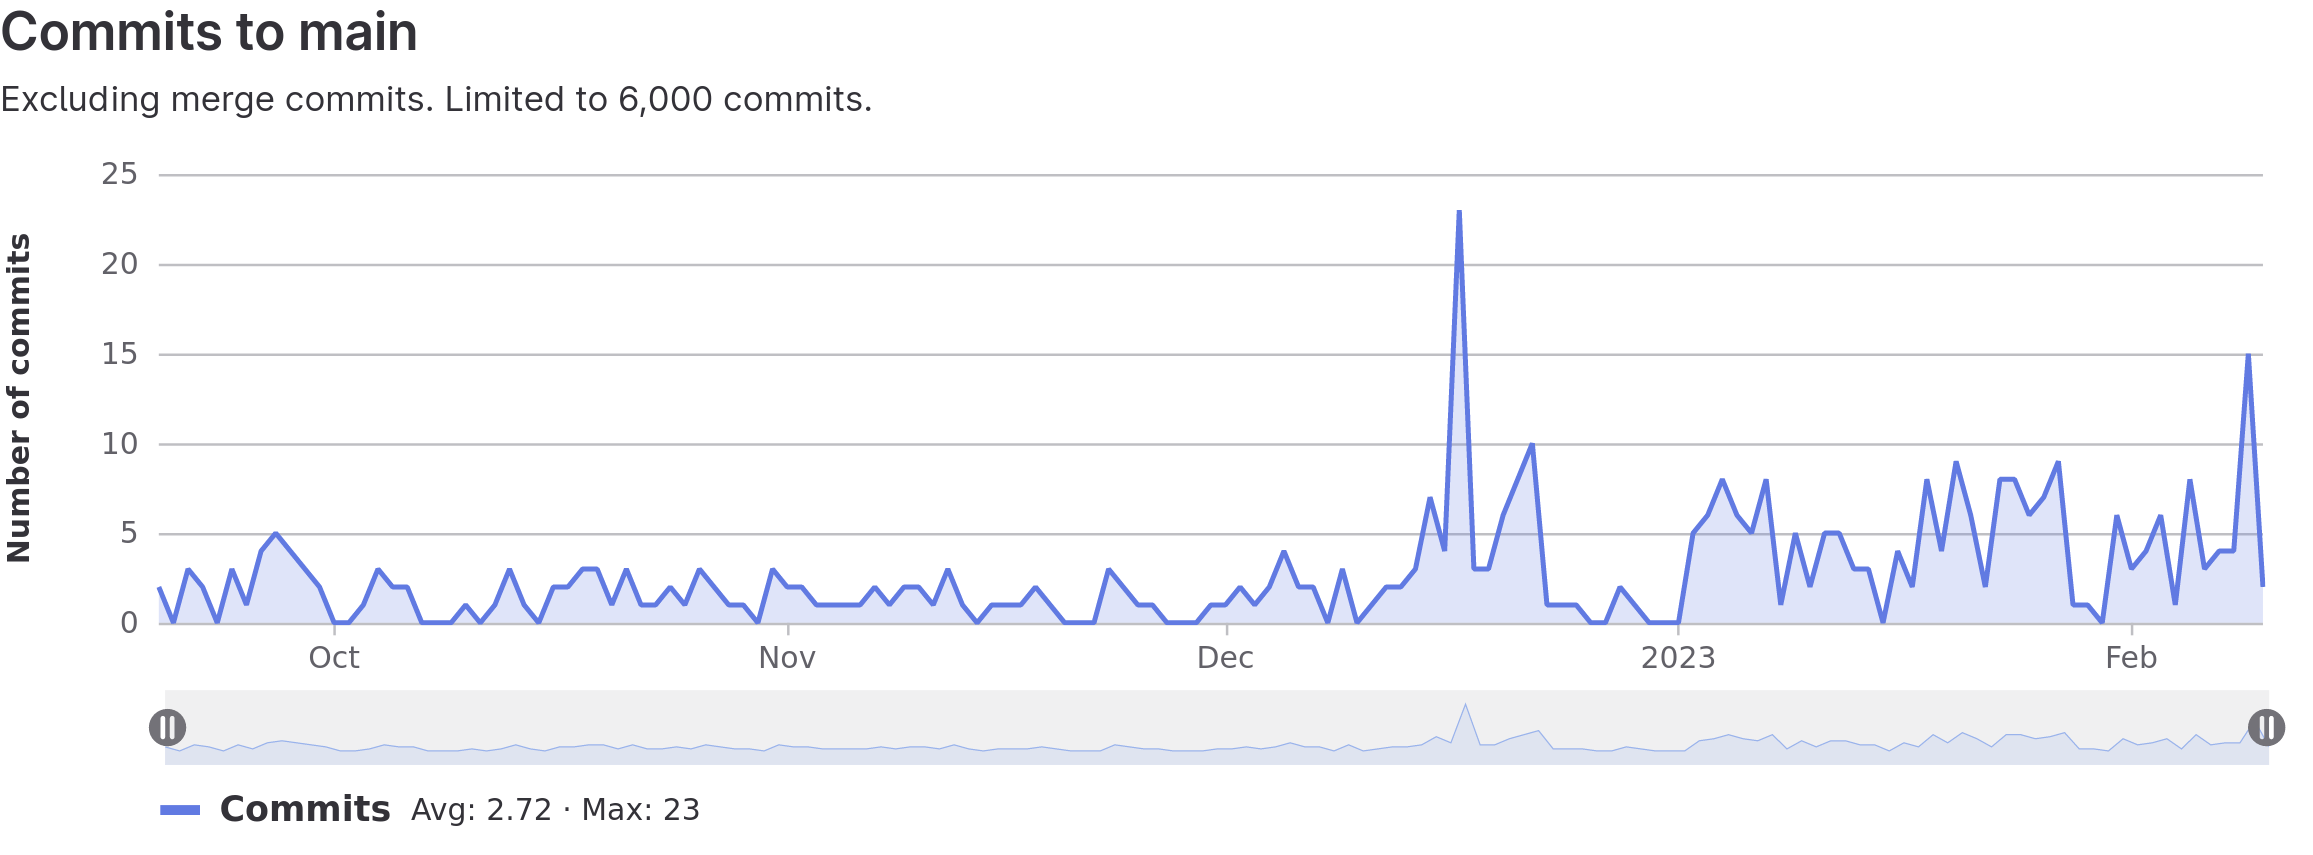
\includegraphics[width=1\textwidth]{03-tail/appendices/repository.png}

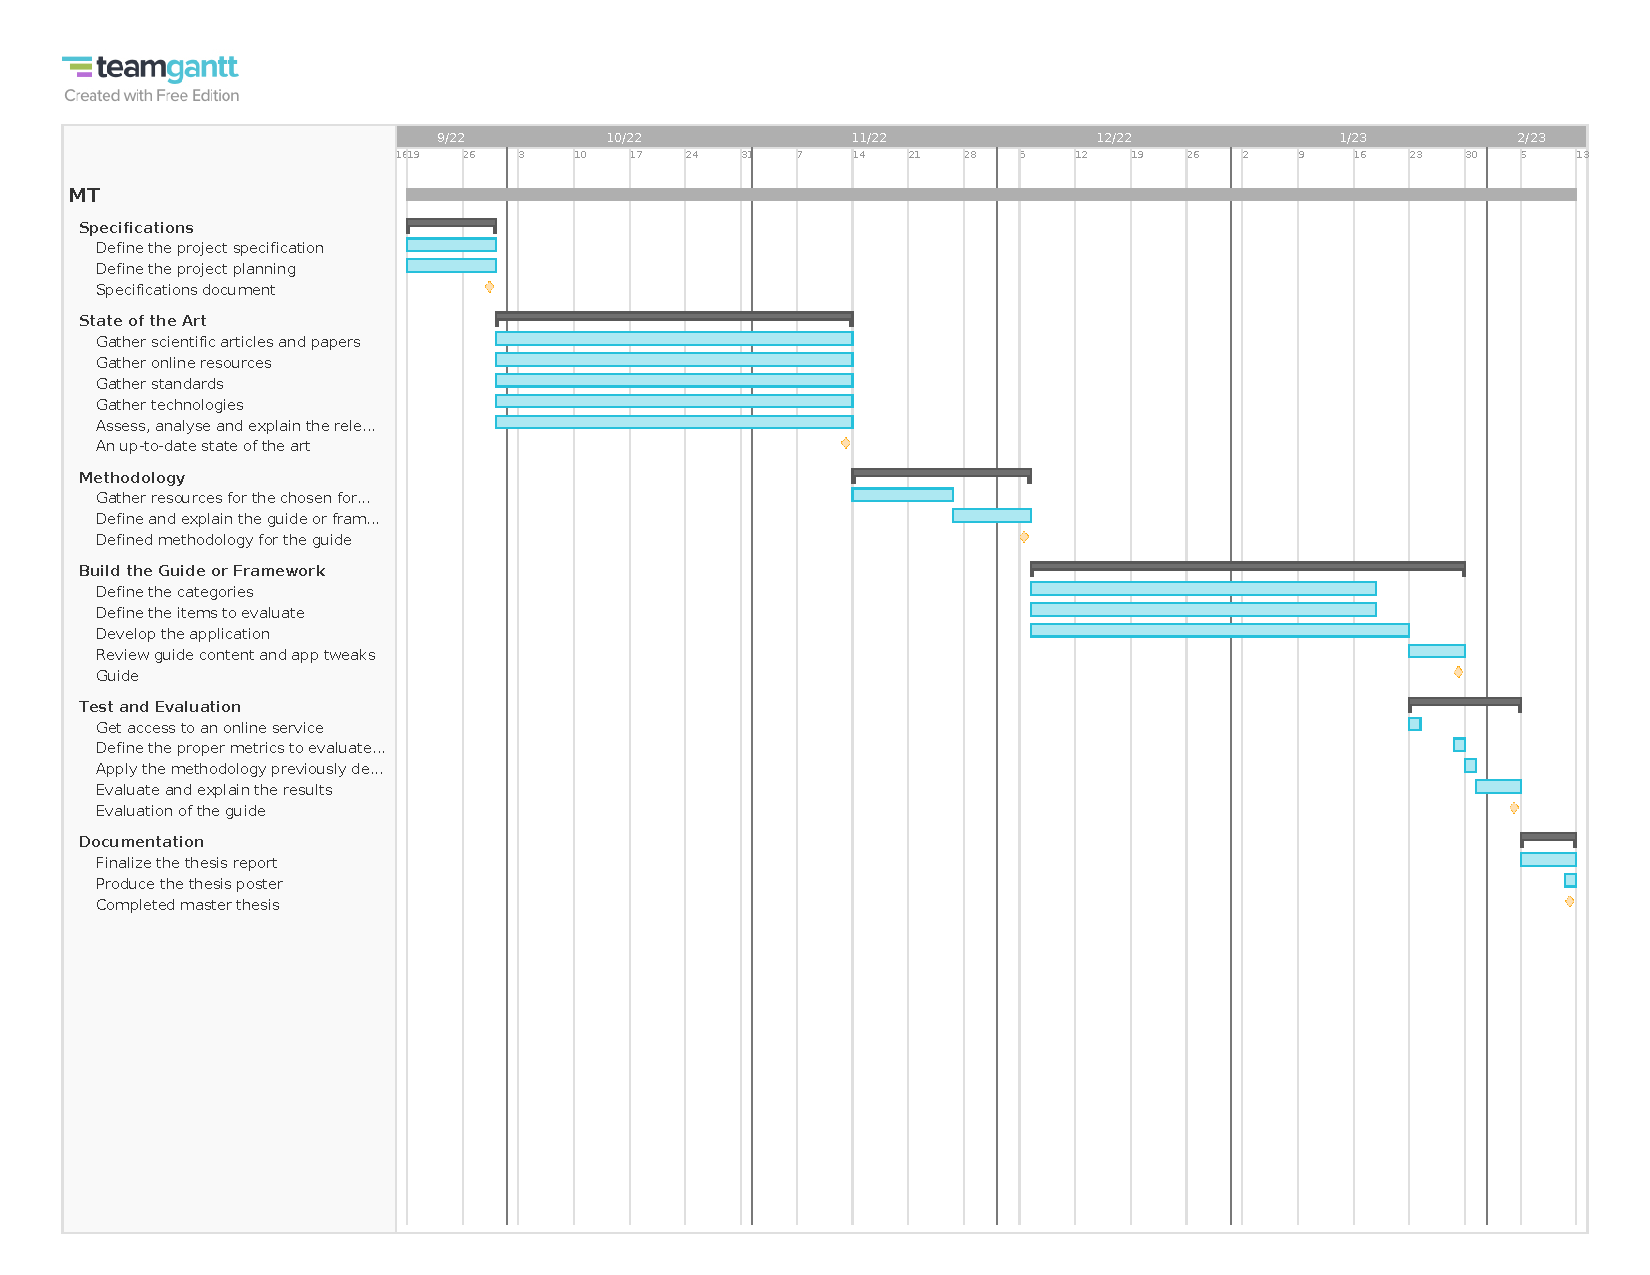
\includepdf[pages={-},angle=90]{03-tail/appendices/gantt_final.pdf}

% -----------------------------------------------------------------------------
\newappendix{Software and Tools}
\label{appendix:software}

This appendix does not list the software dependencies or tools if they have already been presented before in this report.

\subsection*{Office Tools}

All the software and tools used for the administrative or documentation tasks are listed here.

\citeproper{\LaTeX \ Suite - pdfTeX}, used to generate the documents for this project.

\begin{itemize}
	\item Version 3.141592653-2.6-1.40.22 (TeX Live 2021)
	\item Licence pdfTeX copyright, Lesser GNU General Public
\end{itemize}


\citeproper{Zotero}, used to manage the dissertation references.

\begin{itemize}
	\item Version 6.0.13
	\item Licence AGPL-3.0
\end{itemize}


\citeproper{Draw.io}, used to draw the different graphs.

\begin{itemize}
	\item Version 19.0.0
	\item Licence APACHE Licence, version 2.0
\end{itemize}


\citeproper{Microsoft Teams}, used to conduct organizational and follow-up sessions.

\begin{itemize}
	\item Version 1.5.00.10453 (64-bit) (64 bits)
	\item Licence Proprietary
\end{itemize}

\newpage

\subsection*{Development Tools}

All the software and tools used for the development tasks are listed here.

\citeproper{LibreWolf}, used for research, implementation and testing.

\begin{itemize}
	\item Version from 104.0.2-1
	\item Licence MPL-2.0 (d), GNU General Public Licence (GPL) et GNU Lesser General Public Licence (LGPL)
\end{itemize}


\citeproper{ungoogled-chromium}, used for research, implementation and testing.

\begin{itemize}
	\item Version 105.0.5195.125
	\item Licence BSD-3-Clause
\end{itemize}


\citeproper{GitLab}, used to manage the versioning of project resources.

\begin{itemize}
	\item Version GitLab Enterprise Edition 15.3.2-ee
	\item Licence MIT Licence
\end{itemize}


\citeproper{VSCodium}, used to implement \citeproper{JavaScript} software and to redact the \LaTeX documents.

\begin{itemize}
	\item Version 1.71.2
	\item Licence MIT Licence
\end{itemize}


\citeproper{PyCharm Professional}, used to implement the \citeproper{Python} script.

\begin{itemize}
	\item Version 2022.2.4
	\item Licence Copyright © 2010-2022 JetBrains s.r.o.
\end{itemize}


\citeproper{LibreOffice Calc}, used to create the spreadsheet file.

\begin{itemize}
	\item Version 7.4.3.2
	\item Licence MPL-2.0
\end{itemize}